% Options for packages loaded elsewhere
\PassOptionsToPackage{unicode}{hyperref}
\PassOptionsToPackage{hyphens}{url}
\PassOptionsToPackage{dvipsnames,svgnames,x11names}{xcolor}
%
\documentclass[
  letterpaper,
  DIV=11,
  numbers=noendperiod]{scrartcl}

\usepackage{amsmath,amssymb}
\usepackage{lmodern}
\usepackage{iftex}
\ifPDFTeX
  \usepackage[T1]{fontenc}
  \usepackage[utf8]{inputenc}
  \usepackage{textcomp} % provide euro and other symbols
\else % if luatex or xetex
  \usepackage{unicode-math}
  \defaultfontfeatures{Scale=MatchLowercase}
  \defaultfontfeatures[\rmfamily]{Ligatures=TeX,Scale=1}
\fi
% Use upquote if available, for straight quotes in verbatim environments
\IfFileExists{upquote.sty}{\usepackage{upquote}}{}
\IfFileExists{microtype.sty}{% use microtype if available
  \usepackage[]{microtype}
  \UseMicrotypeSet[protrusion]{basicmath} % disable protrusion for tt fonts
}{}
\makeatletter
\@ifundefined{KOMAClassName}{% if non-KOMA class
  \IfFileExists{parskip.sty}{%
    \usepackage{parskip}
  }{% else
    \setlength{\parindent}{0pt}
    \setlength{\parskip}{6pt plus 2pt minus 1pt}}
}{% if KOMA class
  \KOMAoptions{parskip=half}}
\makeatother
\usepackage{xcolor}
\setlength{\emergencystretch}{3em} % prevent overfull lines
\setcounter{secnumdepth}{-\maxdimen} % remove section numbering
% Make \paragraph and \subparagraph free-standing
\ifx\paragraph\undefined\else
  \let\oldparagraph\paragraph
  \renewcommand{\paragraph}[1]{\oldparagraph{#1}\mbox{}}
\fi
\ifx\subparagraph\undefined\else
  \let\oldsubparagraph\subparagraph
  \renewcommand{\subparagraph}[1]{\oldsubparagraph{#1}\mbox{}}
\fi

\usepackage{color}
\usepackage{fancyvrb}
\newcommand{\VerbBar}{|}
\newcommand{\VERB}{\Verb[commandchars=\\\{\}]}
\DefineVerbatimEnvironment{Highlighting}{Verbatim}{commandchars=\\\{\}}
% Add ',fontsize=\small' for more characters per line
\usepackage{framed}
\definecolor{shadecolor}{RGB}{241,243,245}
\newenvironment{Shaded}{\begin{snugshade}}{\end{snugshade}}
\newcommand{\AlertTok}[1]{\textcolor[rgb]{0.68,0.00,0.00}{#1}}
\newcommand{\AnnotationTok}[1]{\textcolor[rgb]{0.37,0.37,0.37}{#1}}
\newcommand{\AttributeTok}[1]{\textcolor[rgb]{0.40,0.45,0.13}{#1}}
\newcommand{\BaseNTok}[1]{\textcolor[rgb]{0.68,0.00,0.00}{#1}}
\newcommand{\BuiltInTok}[1]{\textcolor[rgb]{0.00,0.23,0.31}{#1}}
\newcommand{\CharTok}[1]{\textcolor[rgb]{0.13,0.47,0.30}{#1}}
\newcommand{\CommentTok}[1]{\textcolor[rgb]{0.37,0.37,0.37}{#1}}
\newcommand{\CommentVarTok}[1]{\textcolor[rgb]{0.37,0.37,0.37}{\textit{#1}}}
\newcommand{\ConstantTok}[1]{\textcolor[rgb]{0.56,0.35,0.01}{#1}}
\newcommand{\ControlFlowTok}[1]{\textcolor[rgb]{0.00,0.23,0.31}{#1}}
\newcommand{\DataTypeTok}[1]{\textcolor[rgb]{0.68,0.00,0.00}{#1}}
\newcommand{\DecValTok}[1]{\textcolor[rgb]{0.68,0.00,0.00}{#1}}
\newcommand{\DocumentationTok}[1]{\textcolor[rgb]{0.37,0.37,0.37}{\textit{#1}}}
\newcommand{\ErrorTok}[1]{\textcolor[rgb]{0.68,0.00,0.00}{#1}}
\newcommand{\ExtensionTok}[1]{\textcolor[rgb]{0.00,0.23,0.31}{#1}}
\newcommand{\FloatTok}[1]{\textcolor[rgb]{0.68,0.00,0.00}{#1}}
\newcommand{\FunctionTok}[1]{\textcolor[rgb]{0.28,0.35,0.67}{#1}}
\newcommand{\ImportTok}[1]{\textcolor[rgb]{0.00,0.46,0.62}{#1}}
\newcommand{\InformationTok}[1]{\textcolor[rgb]{0.37,0.37,0.37}{#1}}
\newcommand{\KeywordTok}[1]{\textcolor[rgb]{0.00,0.23,0.31}{#1}}
\newcommand{\NormalTok}[1]{\textcolor[rgb]{0.00,0.23,0.31}{#1}}
\newcommand{\OperatorTok}[1]{\textcolor[rgb]{0.37,0.37,0.37}{#1}}
\newcommand{\OtherTok}[1]{\textcolor[rgb]{0.00,0.23,0.31}{#1}}
\newcommand{\PreprocessorTok}[1]{\textcolor[rgb]{0.68,0.00,0.00}{#1}}
\newcommand{\RegionMarkerTok}[1]{\textcolor[rgb]{0.00,0.23,0.31}{#1}}
\newcommand{\SpecialCharTok}[1]{\textcolor[rgb]{0.37,0.37,0.37}{#1}}
\newcommand{\SpecialStringTok}[1]{\textcolor[rgb]{0.13,0.47,0.30}{#1}}
\newcommand{\StringTok}[1]{\textcolor[rgb]{0.13,0.47,0.30}{#1}}
\newcommand{\VariableTok}[1]{\textcolor[rgb]{0.07,0.07,0.07}{#1}}
\newcommand{\VerbatimStringTok}[1]{\textcolor[rgb]{0.13,0.47,0.30}{#1}}
\newcommand{\WarningTok}[1]{\textcolor[rgb]{0.37,0.37,0.37}{\textit{#1}}}

\providecommand{\tightlist}{%
  \setlength{\itemsep}{0pt}\setlength{\parskip}{0pt}}\usepackage{longtable,booktabs,array}
\usepackage{calc} % for calculating minipage widths
% Correct order of tables after \paragraph or \subparagraph
\usepackage{etoolbox}
\makeatletter
\patchcmd\longtable{\par}{\if@noskipsec\mbox{}\fi\par}{}{}
\makeatother
% Allow footnotes in longtable head/foot
\IfFileExists{footnotehyper.sty}{\usepackage{footnotehyper}}{\usepackage{footnote}}
\makesavenoteenv{longtable}
\usepackage{graphicx}
\makeatletter
\def\maxwidth{\ifdim\Gin@nat@width>\linewidth\linewidth\else\Gin@nat@width\fi}
\def\maxheight{\ifdim\Gin@nat@height>\textheight\textheight\else\Gin@nat@height\fi}
\makeatother
% Scale images if necessary, so that they will not overflow the page
% margins by default, and it is still possible to overwrite the defaults
% using explicit options in \includegraphics[width, height, ...]{}
\setkeys{Gin}{width=\maxwidth,height=\maxheight,keepaspectratio}
% Set default figure placement to htbp
\makeatletter
\def\fps@figure{htbp}
\makeatother
\newlength{\cslhangindent}
\setlength{\cslhangindent}{1.5em}
\newlength{\csllabelwidth}
\setlength{\csllabelwidth}{3em}
\newlength{\cslentryspacingunit} % times entry-spacing
\setlength{\cslentryspacingunit}{\parskip}
\newenvironment{CSLReferences}[2] % #1 hanging-ident, #2 entry spacing
 {% don't indent paragraphs
  \setlength{\parindent}{0pt}
  % turn on hanging indent if param 1 is 1
  \ifodd #1
  \let\oldpar\par
  \def\par{\hangindent=\cslhangindent\oldpar}
  \fi
  % set entry spacing
  \setlength{\parskip}{#2\cslentryspacingunit}
 }%
 {}
\usepackage{calc}
\newcommand{\CSLBlock}[1]{#1\hfill\break}
\newcommand{\CSLLeftMargin}[1]{\parbox[t]{\csllabelwidth}{#1}}
\newcommand{\CSLRightInline}[1]{\parbox[t]{\linewidth - \csllabelwidth}{#1}\break}
\newcommand{\CSLIndent}[1]{\hspace{\cslhangindent}#1}

\usepackage{booktabs}
\usepackage{caption}
\usepackage{longtable}
\KOMAoption{captions}{tableheading}
\makeatletter
\makeatother
\makeatletter
\makeatother
\makeatletter
\@ifpackageloaded{caption}{}{\usepackage{caption}}
\AtBeginDocument{%
\ifdefined\contentsname
  \renewcommand*\contentsname{Table of contents}
\else
  \newcommand\contentsname{Table of contents}
\fi
\ifdefined\listfigurename
  \renewcommand*\listfigurename{List of Figures}
\else
  \newcommand\listfigurename{List of Figures}
\fi
\ifdefined\listtablename
  \renewcommand*\listtablename{List of Tables}
\else
  \newcommand\listtablename{List of Tables}
\fi
\ifdefined\figurename
  \renewcommand*\figurename{Figure}
\else
  \newcommand\figurename{Figure}
\fi
\ifdefined\tablename
  \renewcommand*\tablename{Table}
\else
  \newcommand\tablename{Table}
\fi
}
\@ifpackageloaded{float}{}{\usepackage{float}}
\floatstyle{ruled}
\@ifundefined{c@chapter}{\newfloat{codelisting}{h}{lop}}{\newfloat{codelisting}{h}{lop}[chapter]}
\floatname{codelisting}{Listing}
\newcommand*\listoflistings{\listof{codelisting}{List of Listings}}
\makeatother
\makeatletter
\@ifpackageloaded{caption}{}{\usepackage{caption}}
\@ifpackageloaded{subcaption}{}{\usepackage{subcaption}}
\makeatother
\makeatletter
\@ifpackageloaded{tcolorbox}{}{\usepackage[many]{tcolorbox}}
\makeatother
\makeatletter
\@ifundefined{shadecolor}{\definecolor{shadecolor}{rgb}{.97, .97, .97}}
\makeatother
\makeatletter
\makeatother
\ifLuaTeX
  \usepackage{selnolig}  % disable illegal ligatures
\fi
\IfFileExists{bookmark.sty}{\usepackage{bookmark}}{\usepackage{hyperref}}
\IfFileExists{xurl.sty}{\usepackage{xurl}}{} % add URL line breaks if available
\urlstyle{same} % disable monospaced font for URLs
\hypersetup{
  pdftitle={Hello, Quarto},
  colorlinks=true,
  linkcolor={blue},
  filecolor={Maroon},
  citecolor={Blue},
  urlcolor={Blue},
  pdfcreator={LaTeX via pandoc}}

\title{Hello, Quarto}
\author{}
\date{}

\begin{document}
\maketitle
\ifdefined\Shaded\renewenvironment{Shaded}{\begin{tcolorbox}[breakable, sharp corners, interior hidden, frame hidden, borderline west={3pt}{0pt}{shadecolor}, boxrule=0pt, enhanced]}{\end{tcolorbox}}\fi

\hypertarget{r-package-jmpwashdata}{%
\section{R Package jmpwashdata}\label{r-package-jmpwashdata}}

For this analysis we will use the \textbf{jmpwashdata} R Package by
(Dickinson 2021). The package contains all data compiled by the
\href{https://washdata.org}{WHO/UNICEF Joint Monitoring Programme
(JMP)}.

\begin{Shaded}
\begin{Highlighting}[]
\FunctionTok{library}\NormalTok{(jmpwashdata)}
\FunctionTok{library}\NormalTok{(tidyverse)}
\FunctionTok{library}\NormalTok{(gt)}
\FunctionTok{library}\NormalTok{(ggthemes)}
\end{Highlighting}
\end{Shaded}

\hypertarget{world-bank-income-groups}{%
\section{World Bank income groups}\label{world-bank-income-groups}}

We will also use the World Bank income classification for 218 countries.
This data was downloaded and stored as an XLSX file using an R script in
\texttt{src}.

\begin{Shaded}
\begin{Highlighting}[]
\NormalTok{income\_groups\_df }\SpecialCharTok{\%\textgreater{}\%} 
  \FunctionTok{count}\NormalTok{(income\_group) }\SpecialCharTok{\%\textgreater{}\%} 
  \FunctionTok{gt}\NormalTok{()}
\end{Highlighting}
\end{Shaded}

\begin{longtable}{cr}
\toprule
income\_group & n \\ 
\midrule
High income & 81 \\ 
Upper middle income & 54 \\ 
Lower middle income & 54 \\ 
Low income & 28 \\ 
NA & 1 \\ 
\bottomrule
\end{longtable}

\hypertarget{basic-sanitation-gdp}{%
\section{Basic Sanitation \& GDP}\label{basic-sanitation-gdp}}

Data for the most recent year, basic sanitation in urban areas,
calculate urban population, and join income groups.

\begin{Shaded}
\begin{Highlighting}[]
\CommentTok{\# Perform data manipulation operations on the jmp\_wld\_sanitation data frame}
\NormalTok{jmp\_wld\_sanitation\_gdp\_income }\OtherTok{\textless{}{-}}\NormalTok{ jmp\_wld\_sanitation }\SpecialCharTok{|\textgreater{}} 
  \CommentTok{\# Filter the rows where the year column is equal to the maximum year value}
  \FunctionTok{filter}\NormalTok{(year }\SpecialCharTok{==} \FunctionTok{max}\NormalTok{(year)) }\SpecialCharTok{|\textgreater{}} 
  \CommentTok{\# Select the columns from name to prop\_u and the san\_bas\_u column}
  \FunctionTok{select}\NormalTok{(name}\SpecialCharTok{:}\NormalTok{prop\_u, san\_bas\_u) }\SpecialCharTok{|\textgreater{}} 
  \CommentTok{\# Create a new column named pop\_u}
  \FunctionTok{mutate}\NormalTok{(}\AttributeTok{pop\_u =}\NormalTok{ pop\_n }\SpecialCharTok{*} \DecValTok{1000} \SpecialCharTok{*}\NormalTok{ prop\_u }\SpecialCharTok{/} \DecValTok{100}\NormalTok{) }\SpecialCharTok{|\textgreater{}} 
  \CommentTok{\# Drop the pop\_n and prop\_u columns}
  \FunctionTok{select}\NormalTok{(}\SpecialCharTok{{-}}\NormalTok{pop\_n, }\SpecialCharTok{{-}}\NormalTok{prop\_u) }\SpecialCharTok{|\textgreater{}} 
  \CommentTok{\# Perform a left join with the income\_groups\_df data frame}
  \FunctionTok{left\_join}\NormalTok{(income\_groups\_df) }\SpecialCharTok{|\textgreater{}} 
  \CommentTok{\# Drop the rows that have missing values in the san\_bas\_u \& income\_group cols}
  \FunctionTok{drop\_na}\NormalTok{(san\_bas\_u, income\_group)}
\end{Highlighting}
\end{Shaded}

\begin{verbatim}
Joining with `by = join_by(iso3)`
\end{verbatim}

\hypertarget{basic-sanitation-uganda}{%
\section{Basic Sanitation Uganda}\label{basic-sanitation-uganda}}

\begin{Shaded}
\begin{Highlighting}[]
\CommentTok{\# Create a vector of color codes}
\NormalTok{color\_scale\_sanitation }\OtherTok{\textless{}{-}} \FunctionTok{c}\NormalTok{(}\StringTok{"\#8cce8f"}\NormalTok{, }\StringTok{"\#fff381"}\NormalTok{, }\StringTok{"\#ffda5a"}\NormalTok{, }\StringTok{"\#ffbc02"}\NormalTok{)}

\CommentTok{\# Create a vector of sanitation indicators}
\NormalTok{fct\_sanitation }\OtherTok{\textless{}{-}} \FunctionTok{c}\NormalTok{(}\StringTok{"basic"}\NormalTok{, }\StringTok{"limited"}\NormalTok{, }\StringTok{"unimproved"}\NormalTok{, }\StringTok{"open defecation"}\NormalTok{)}

\CommentTok{\# Perform data manipulation operations on the jmp\_wld\_sanitation data frame}
\NormalTok{jmp\_uga\_sanitation }\OtherTok{\textless{}{-}}\NormalTok{ jmp\_wld\_sanitation }\SpecialCharTok{|\textgreater{}} 
  \CommentTok{\# Filter the rows where the iso3 column is equal to "UGA" and the year column }
  \CommentTok{\# is equal to 2000 or 2020}
  \FunctionTok{filter}\NormalTok{(iso3 }\SpecialCharTok{==} \StringTok{"UGA"}\NormalTok{) }\SpecialCharTok{|\textgreater{}} 
  \FunctionTok{filter}\NormalTok{(year }\SpecialCharTok{==} \DecValTok{2000} \SpecialCharTok{|}\NormalTok{ year }\SpecialCharTok{==} \DecValTok{2020}\NormalTok{) }\SpecialCharTok{|\textgreater{}} 
  \CommentTok{\# Select the name, iso3, year, and columns from san\_bas\_n to san\_od\_n}
  \FunctionTok{select}\NormalTok{(name, iso3, year, san\_bas\_n}\SpecialCharTok{:}\NormalTok{san\_od\_n) }\SpecialCharTok{|\textgreater{}} 
  \CommentTok{\# Reshape the data frame from wide to long format}
  \FunctionTok{pivot\_longer}\NormalTok{(}\AttributeTok{cols =}\NormalTok{ san\_bas\_n}\SpecialCharTok{:}\NormalTok{san\_od\_n, }
               \AttributeTok{names\_to =} \StringTok{"indicator"}\NormalTok{, }
               \AttributeTok{values\_to =} \StringTok{"percent"}\NormalTok{) }\SpecialCharTok{|\textgreater{}} 
  \CommentTok{\# Rename the indicator column based on the values of the san\_bas\_n to san\_od\_n}
  \CommentTok{\# columns}
  \FunctionTok{mutate}\NormalTok{(}\AttributeTok{indicator =} \FunctionTok{case\_when}\NormalTok{(}
\NormalTok{    indicator }\SpecialCharTok{==} \StringTok{"san\_bas\_n"} \SpecialCharTok{\textasciitilde{}} \StringTok{"basic"}\NormalTok{,}
\NormalTok{    indicator }\SpecialCharTok{==} \StringTok{"san\_lim\_n"} \SpecialCharTok{\textasciitilde{}} \StringTok{"limited"}\NormalTok{,}
\NormalTok{    indicator }\SpecialCharTok{==} \StringTok{"san\_unimp\_n"} \SpecialCharTok{\textasciitilde{}} \StringTok{"unimproved"}\NormalTok{,}
\NormalTok{    indicator }\SpecialCharTok{==} \StringTok{"san\_od\_n"} \SpecialCharTok{\textasciitilde{}} \StringTok{"open defecation"}
\NormalTok{  )) }\SpecialCharTok{|\textgreater{}} 
  \CommentTok{\# Convert the indicator column to a factor with levels specified by the }
  \CommentTok{\# fct\_sanitation vector}
  \FunctionTok{mutate}\NormalTok{(}\AttributeTok{indicator =} \FunctionTok{factor}\NormalTok{(indicator, }\AttributeTok{level =}\NormalTok{ fct\_sanitation))}
\end{Highlighting}
\end{Shaded}

\hypertarget{income}{%
\section{Income}\label{income}}

Figure~\ref{fig-san-bas-u-income} is a box- and jitterplot of countries
with percentages of populations with access to basic sanitation in 2020
grouped by income classifications.

\begin{Shaded}
\begin{Highlighting}[]
\FunctionTok{ggplot}\NormalTok{(}\AttributeTok{data =}\NormalTok{ jmp\_wld\_sanitation\_gdp\_income,}
       \AttributeTok{mapping =} \FunctionTok{aes}\NormalTok{(}\AttributeTok{x =}\NormalTok{ income\_group, }
                     \AttributeTok{y =}\NormalTok{ san\_bas\_u, }
                     \AttributeTok{color =}\NormalTok{ income\_group)) }\SpecialCharTok{+}
  \FunctionTok{geom\_boxplot}\NormalTok{(}\AttributeTok{outlier.shape =} \ConstantTok{NA}\NormalTok{) }\SpecialCharTok{+}
  \FunctionTok{geom\_jitter}\NormalTok{(}\AttributeTok{width =} \FloatTok{0.1}\NormalTok{, }\AttributeTok{size =} \DecValTok{4}\NormalTok{, }\AttributeTok{alpha =} \FloatTok{0.5}\NormalTok{) }\SpecialCharTok{+}
  \FunctionTok{labs}\NormalTok{(}\AttributeTok{x =} \ConstantTok{NULL}\NormalTok{, }\AttributeTok{y =} \StringTok{"percent"}\NormalTok{) }\SpecialCharTok{+}
  \FunctionTok{scale\_color\_colorblind}\NormalTok{() }\SpecialCharTok{+}
  \FunctionTok{theme\_minimal}\NormalTok{(}\AttributeTok{base\_size =} \DecValTok{16}\NormalTok{) }\SpecialCharTok{+}
  \FunctionTok{theme}\NormalTok{(}\AttributeTok{legend.position =} \StringTok{"none"}\NormalTok{)}
\end{Highlighting}
\end{Shaded}

\begin{figure}[H]

{\centering 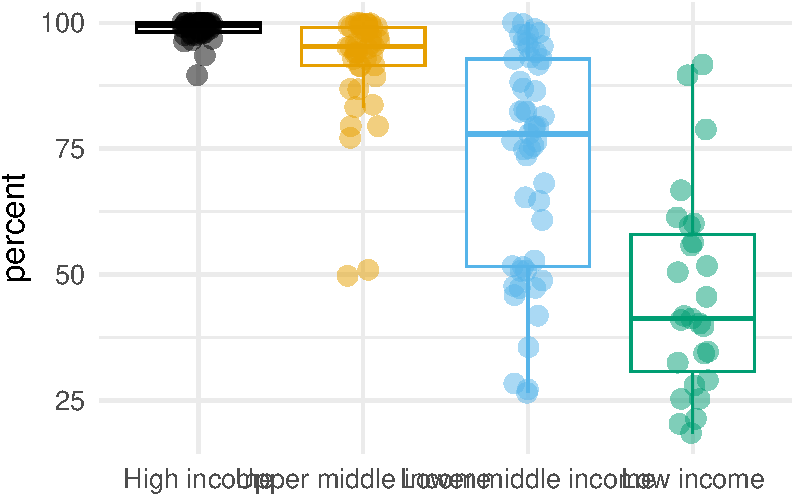
\includegraphics{index_files/figure-pdf/fig-san-bas-u-income-1.pdf}

}

\caption{\label{fig-san-bas-u-income}Access to sanitation (urban) in
2020 by income classifications.}

\end{figure}

\hypertarget{regions}{%
\section{Regions}\label{regions}}

Table~\ref{tbl-reg-sanitation} shows urban sanitation indicators for
global regions in 2020.

\begin{Shaded}
\begin{Highlighting}[]
\NormalTok{jmp\_reg\_sanitation }\SpecialCharTok{|\textgreater{}} 
  \FunctionTok{filter}\NormalTok{(year }\SpecialCharTok{==} \FunctionTok{max}\NormalTok{(year)) }\SpecialCharTok{|\textgreater{}} 
  \FunctionTok{filter}\NormalTok{(}\SpecialCharTok{!}\FunctionTok{str\_detect}\NormalTok{(region, }\StringTok{"income"}\NormalTok{)) }\SpecialCharTok{|\textgreater{}} 
  \FunctionTok{select}\NormalTok{(region, san\_bas\_u}\SpecialCharTok{:}\NormalTok{san\_od\_u) }\SpecialCharTok{|\textgreater{}} 
  \FunctionTok{drop\_na}\NormalTok{() }\SpecialCharTok{|\textgreater{}} 
  \FunctionTok{gt}\NormalTok{(}\AttributeTok{rowname\_col =} \StringTok{"region"}\NormalTok{) }\SpecialCharTok{|\textgreater{}} 
  \FunctionTok{cols\_label}\NormalTok{(}
    \AttributeTok{san\_bas\_u =} \FunctionTok{md}\NormalTok{(}\StringTok{"**basic**"}\NormalTok{),}
    \AttributeTok{san\_lim\_u =} \FunctionTok{md}\NormalTok{(}\StringTok{"**limited**"}\NormalTok{),}
    \AttributeTok{san\_unimp\_u =} \FunctionTok{md}\NormalTok{(}\StringTok{"**unimproved**"}\NormalTok{),}
    \AttributeTok{san\_od\_u =} \FunctionTok{md}\NormalTok{(}\StringTok{"**open defecation**"}\NormalTok{)}
\NormalTok{  ) }\SpecialCharTok{|\textgreater{}} 
  \FunctionTok{fmt\_percent}\NormalTok{(}\AttributeTok{columns =}\NormalTok{ san\_bas\_u}\SpecialCharTok{:}\NormalTok{san\_od\_u,}
              \AttributeTok{decimals =} \DecValTok{0}\NormalTok{, }
              \AttributeTok{scale\_values =} \ConstantTok{FALSE}\NormalTok{) }
\end{Highlighting}
\end{Shaded}

\hypertarget{tbl-reg-sanitation}{}
\begin{longtable}{l|rrrr}
\caption{\label{tbl-reg-sanitation}Urban sanitation indicators for glabal regions. }\tabularnewline

\toprule
\multicolumn{1}{l}{} & \textbf{basic} & \textbf{limited} & \textbf{unimproved} & \textbf{open defecation} \\ 
\midrule
Central and Southern Asia & $79\%$ & $17\%$ & $3\%$ & $1\%$ \\ 
Eastern and South-Eastern Asia & $95\%$ & $3\%$ & $2\%$ & $1\%$ \\ 
Europe and Northern America & $99\%$ & $1\%$ & $1\%$ & $0\%$ \\ 
Latin America and the Caribbean & $93\%$ & $4\%$ & $3\%$ & $0\%$ \\ 
Northern Africa and Western Asia & $95\%$ & $2\%$ & $2\%$ & $0\%$ \\ 
Oceania & $71\%$ & $9\%$ & $17\%$ & $3\%$ \\ 
Sub-Saharan Africa & $46\%$ & $32\%$ & $17\%$ & $5\%$ \\ 
Fragile or Extremely Fragile & $62\%$ & $22\%$ & $13\%$ & $3\%$ \\ 
Least Developed Countries & $48\%$ & $29\%$ & $20\%$ & $4\%$ \\ 
Landlocked Developing Countries & $62\%$ & $22\%$ & $14\%$ & $2\%$ \\ 
Small Island Developing States & $83\%$ & $10\%$ & $5\%$ & $2\%$ \\ 
World & $88\%$ & $8\%$ & $3\%$ & $1\%$ \\ 
\bottomrule
\end{longtable}

\hypertarget{uganda}{%
\section{Uganda}\label{uganda}}

Figure~\ref{fig-san-uga} shows the sanitation ladder for Uganda.

\begin{Shaded}
\begin{Highlighting}[]
\FunctionTok{ggplot}\NormalTok{(}\AttributeTok{data =}\NormalTok{ jmp\_uga\_sanitation, }
       \AttributeTok{mapping =} \FunctionTok{aes}\NormalTok{(}\AttributeTok{x =}\NormalTok{ year, }
                     \AttributeTok{y =}\NormalTok{ percent, }
                     \AttributeTok{fill =}\NormalTok{ indicator)) }\SpecialCharTok{+}
  \FunctionTok{geom\_area}\NormalTok{() }\SpecialCharTok{+}
  \FunctionTok{labs}\NormalTok{(}\AttributeTok{title =} \StringTok{"Uganda: sanitation ladder (national)"}\NormalTok{,}
       \AttributeTok{x =} \ConstantTok{NULL}\NormalTok{, }\AttributeTok{y =} \StringTok{"percent"}\NormalTok{, }\AttributeTok{fill =} \StringTok{"indicators"}\NormalTok{) }\SpecialCharTok{+}
  \FunctionTok{scale\_fill\_manual}\NormalTok{(}\AttributeTok{values =}\NormalTok{ color\_scale\_sanitation) }\SpecialCharTok{+}
  \FunctionTok{scale\_x\_continuous}\NormalTok{(}\AttributeTok{breaks =} \FunctionTok{c}\NormalTok{(}\DecValTok{2000}\NormalTok{, }\DecValTok{2020}\NormalTok{)) }\SpecialCharTok{+}
  \FunctionTok{theme\_minimal}\NormalTok{(}\AttributeTok{base\_size =} \DecValTok{16}\NormalTok{) }\SpecialCharTok{+}
  \FunctionTok{theme}\NormalTok{(}\AttributeTok{panel.grid.minor =} \FunctionTok{element\_blank}\NormalTok{()) }
\end{Highlighting}
\end{Shaded}

\begin{figure}[H]

{\centering 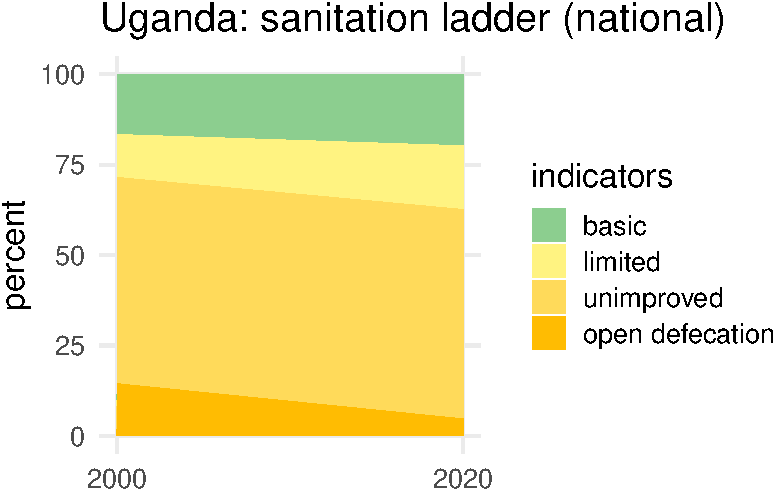
\includegraphics{index_files/figure-pdf/fig-san-uga-1.pdf}

}

\caption{\label{fig-san-uga}Sanitation indicators for Uganda on a
national level.}

\end{figure}

\hypertarget{they-told-you-so}{%
\section*{They told you so}\label{they-told-you-so}}
\addcontentsline{toc}{section}{They told you so}

\hypertarget{refs}{}
\begin{CSLReferences}{1}{0}
\leavevmode\vadjust pre{\hypertarget{ref-jmpwashdata}{}}%
Dickinson, Nicolas. 2021. {``Jmpwashdata: WHO/UNICEF Joint Monitoring
Programme Water and Sanitation Data.''}

\end{CSLReferences}



\end{document}
